\title{Лекция 18\\Представление в базе знаний процессов и действий}
\author[]{Шункевич Д.В.}
\institute[]{Белорусский государственный университет информатики и радиоэлектроники}

\begin{frame}
	\titlepage
\end{frame}

\begin{frame}{\\Содержание лекции}
	\topline
	\justifying
	Понятие процесса, воздействия, действия. Описание действий в семантической памяти, элементарные события в семантической памяти. Классификация действий, в том числе выполняемых в семантической памяти. Отношения, заданные на множестве действий. Контекст выполнения действия. Начальная и конечная ситуация процесса. 
\end{frame}

\begin{frame}{\\Понятие процесса}
\topline
\justifying
\begin{SCn}
	\scnheader{структура}
	\begin{scnrelfromset}{разбиение}
		\scnitem{процесс}
		\begin{scnindent}
			\scnidtf{динамическая структура}
			\scnidtf{нестационарная структура}
		\end{scnindent}
		\scnitem{статическая структура}
		\begin{scnindent}
			\scnidtf{стационарная структура}
			\scnidtf{структура, не изменяющаяся во времени}
		\end{scnindent}
	\end{scnrelfromset}
\end{SCn}

Процессом в ostis-системах называется процесс, связанный с преобразованием некоторой временной сущности из одного состояния в другое (с переходом от одной ситуации к другой).
\end{frame}

\begin{frame}{\\Понятие процесса}
\topline
\justifying	

    Каждый \textbf{\textit{процесс}} определяется возникновением или исчезновением связей, связывающих как заданную \textit{временную сущность} с другими сущностями, так и части указанной \textit{временной сущности} с другими сущностями.\\
    Многим \textit{\textbf{процессам}} можно поставить в соответствие \textit{ситуацию}, которая является его \textit{начальной ситуацией*} и ситуацию, являющейся его \textit{конечной ситуацией*} (указать ситуации, переход между которыми осуществляется в ходе процесса).\\
    \bigskip
    \textit{Процесс} представляет собой изменяющуюся во времени динамическую структуру, полностью представить его в БЗ в общем случае невозможно. Однако, можно ввести sc-элемент, обозначающий конкретный процесс с описанием его декомпозиции на более частные, или описать ситуации, соответствующие его состоянием в разные моменты времени.
\end{frame}

\begin{frame}{\\Понятие воздействия}
\topline
\justifying	

 \begin{SCn}
	\scnheader{воздействие}
	\scnidtf{\textit{процесс} воздействия одной сущности (или некоторого множества \textit{сущностей}) на другую \textit{сущность} (или на некоторое множество других \textit{сущностей})}
	\scnidtf{\textit{процесс}, в котором могут быть явно выделены хотя бы одна воздействующая сущность (\textit{субъект\scnrolesign}) и хотя бы одна \textit{сущность}, на которую осуществляется воздействие (\textit{объект\scnrolesign})}
	\scnidtf{акция}
	\scnsubset{процесс}
	\begin{scnindent}
		\scnidtf{динамическая структура}
	\end{scnindent}

\end{SCn}
\end{frame}

\begin{frame}{\\Участники воздействия}
\topline
\justifying	
\begin{SCn}	
    \scnheader{субъект}
	\scnidtf{активная сущность}
	\scnsubset{сущность}
	\scnidtftext{часто используемый sc-идентификатор}{индивид}
	
    \scnheader{субъект\scnrolesign}
	\scnidtf{воздействующая сущность\scnrolesign}
	\scnidtf{сущность, создающая \textit{причину} изменений другой сущности (объекта)\scnrolesign}

	\scnheader{объект\scnrolesign}
	\scnidtf{воздействуемая сущность\scnrolesign}
	\scnidtf{сущность, являющаяся в рамках заданного воздействия исходным условием (аргументом), необходимым для выполнения этого воздействия\scnrolesign}
\end{SCn}
\end{frame}

\begin{frame}{}
\topline
\justifying	
    Каждому \textit{воздействию} может быть поставлен в соответствие (1) некоторый \textit{субъект\scnrolesign}, то есть сущность, осуществляющая \textit{воздействие} (в частности, это может быть некоторое физическое поле), и (2) некоторый \textit{объект\scnrolesign}, то есть сущность, на которую воздействие направлено. Если \textit{воздействие} связано с \textit{материальной сущностью}, то его объектом является либо сама эта \textit{материальная сущность}, либо некоторая ее пространственная часть.
\end{frame}

\begin{frame}{}
\topline
\justifying	

Поскольку \textit{воздействия} являются частным видом \textit{процессов}, воздействиями наследуются все свойства \textit{процессов}. В частности, используются все \textit{параметры}, заданные на множестве \textit{процессов}, например, \textit{длительность*}, \textit{момент начала процесса*}, \textit{момент завершения процесса\scnsupergroupsign}.

\bigskip

Также, так как воздействие является процессом и, соответственно, представляет собой \textit{динамическую структуру}, то и знак \textit{субъекта воздействия\scnrolesign}, и знак \textit{объекта воздействия\scnrolesign} являются элементами данной структуры. В связи с этим можно рассматривать отношения \textit{субъект воздействия\scnrolesign} и \textit{объект воздействия\scnrolesign} как \textit{ролевые отношения}. Данный факт не запрещает вводить аналогичные \textit{неролевые отношения}, однако это нецелесообразно.
\end{frame}

\begin{frame}{\\Понятие действия}
\topline
\justifying	
\vspace{10mm}
 \begin{SCn}
	\scnheader{действие}
	\scnidtf{\textit{воздействие}, в котором \textit{субъект\scnrolesign} осуществляет \textit{воздействие} целенаправленно, то есть в соответствии с некоторой \textit{целью*}}
	\scnidtf{целенаправленное воздействие, выполняемое одним или несколькими субъектами (кибернетическими системами) с возможным применением некоторых инструментов}
	\scnidtf{акт}
	\scnidtf{операция}
	\scnidtf{осознанное воздействие}
	\scnidtf{активное воздействие}
	\scnsubset{воздействие}
	\begin{scnindent}
		\scnsubset{процесс}
	\end{scnindent}
 \scnidtf{целенаправленный (\scnqq{осознанный}) процесс, выполняемый (управляемый, реализуемый) неким субъектом}
\end{SCn}
\end{frame}

\begin{frame}{}
\begin{SCn}
	\scnidtf{работа}
	\scnidtf{процесс решения некоторой задачи}
	\scnidtf{процесс достижения некоторой цели}
	\scnidtf{целостный фрагмент некоторой деятельности}
	\scnidtf{целенаправленный процесс, управляемый некоторым субъектом}
	\scnidtf{процесс выполнения некоторого действия некоторым субъектом (исполнителем) над некоторыми объектами}
	
	\scnheader{цель*}
	\scnidtf{целевая ситуация*}
	\scnsubset{спецификация*}
	\scnidtf{описание того, что требуется получить (какая ситуация должна быть достигнута) в результате выполнения заданного (специфицируемого) действия*}
\end{SCn}
\end{frame}

\begin{frame}{}
\justifying
\vspace{10mm}
Каждое \textit{действие}, выполняемое тем или иным \textit{субъектом}, трактуется как процесс решения некоторой задачи, то есть процесс достижения заданной \textit{цели*} в заданных условиях, и, следовательно, выполняется целенаправленно. При этом явное указание \textit{действия} и его связи с конкретной задачей может не всегда присутствовать в памяти. Некоторые \textit{задачи} могут решаться определенными субъектами перманентно, например, оптимизация \textit{базы знаний}, поиск некорректностей и так далее и для подобных задач не всегда есть необходимость явно вводить \textit{структуру}, являющуюся формулировкой \textit{задачи}.

Каждое \textit{действие} может обозначать сколь угодно малое преобразование, осуществляемое во внешней среде либо в памяти некоторой \textit{кибернетической системы}, однако в памяти явно вводятся знаки только тех \textit{действий}, для которых есть необходимость явно хранить в памяти их спецификацию в течение некоторого времени.
\end{frame}

\begin{frame}{Элементарные события в семантической памяти}
\topline
\justifying
\vspace{10mm}

\textit{событием} называется процесс, длительность выполнения которого считается несущественной. Элементарным событием в sc-памяти называется событие, в результате выполнения которого изменяется состояние лишь одного элемента.
Элементарные события в sc-памяти:
\begin{textitemize}
    \item событие добавления sc-дуги, выходящей из заданного sc-элемента
    \item событие добавления sc-дуги, входящей в заданный sc-элемент
    \item событие добавления sc-ребра, инцидентного заданному sc-элементу
    \item событие удаления sc-дуги, выходящей из заданного sc-элемента
    \item событие удаления sc-дуги, входящей в заданный sc-элемент
    \item событие удаления sc-ребра, инцидентного заданному sc-элементу
    \item событие удаления sc-элемента
    \item событие изменения содержимого файла
\end{textitemize}
\end{frame}

\begin{frame}{\\Классификация действий}
\topline
\justifying

Класс действий имеет разбиение по следующим признакам:
\begin{textitemize}
	\item место выполнения действия;
	\item функциональная сложность действия;
	\item многоагентность выполнения действия;
	\item текущее состояние действия.
\end{textitemize}
Далее рассмотрим разбиение по каждому признаку по отдельности
\end{frame}

\begin{frame}{Классификация действий по \\признаку места выполнения}
\topline
\justifying
\vspace{5mm}
    \begin{SCn}
	\scnheader{действие}
	\scnrelfrom{разбиение}{Типология классов действий по признаку места выполнения действия}
	\begin{scnindent}
		\begin{scneqtoset}
			\scnitem{информационное действие}
			\begin{scnindent}
				\scnidtf{действие, выполняемое в памяти субъекта действия}
				\scnidtf{действие, выполняемое в памяти}
				\scnidtf{действие кибернетической системы, направленное на обработку информации, хранимой в ее памяти}
			\end{scnindent}
			\scnitem{поведенческое действие}
			\begin{scnindent}
				\scnidtf{действие, выполняемое во внешней среде субъекта действия}
			\end{scnindent}
			\scnitem{рецепторное действие}
			\begin{scnindent}
				\scnidtf{сенсорное действие}
			\end{scnindent}
			\scnitem{эффекторное действие}
		\end{scneqtoset}
	\end{scnindent}
\end{SCn}
\end{frame}

\begin{frame}{}
\topline
\justifying
\vspace{10mm}

\textit{информационное действие} -- действие, направленное на обработку информации, хранимой в памяти кибернетической системы. Результатом выполнения является некоторое новое состояние памяти системы, достигнутое исключительно путём преобразования информации, хранящейся в памяти системы.

\bigskip

\textit{поведенческое действие} -- действие, направленное на изменение состояния внешней среды. Под внешней средой понимаются и компоненты системы, внешние с точки зрения памяти, не являющиеся хранимыми в ней информационными конструкциями. К ним можно отнести различные манипуляторы, средства воздействия системы на внешний мир. К поведенческим задачам можно отнести изменение состояния механической конечности робота, вывод информации на экран и другое.
\end{frame}

\begin{frame}{}
\topline
\justifying
\vspace{10mm}

\textit{рецепторное действие} -- каждое рецепторное действие обозначает класс действий, которые осуществляют преобразования в памяти субъекта действия под воздействием внешней среды.

\bigskip

\textit{эффекторное действие} -- каждое эффекторное действие обозначает класс действий, которые осуществляют преобразования внешней среды под воздействием памяти субъекта воздействия.
\end{frame}

\begin{frame}{Классификация действий по \\признаку функциональной сложности}
\topline
\justifying

\begin{SCn}
\scnheader{действие}
\scnrelfrom{разбиение}{Типология классов действий по признаку функциональной сложности действия}
\begin{scnindent}
	\begin{scneqtoset}
		\scnitem{атомарное действие}
		\begin{scnindent}
			\scnidtf{элементарное действие}
		   	\scntext{пояснение}{Выполняется одним индивидуальным субъектом и не включает в себя выполнение каких-либо дочерних действий.}
    	\end{scnindent}
		\scnitem{неатомарное действие}
		\begin{scnindent}
			\scnidtf{неэлементарное действие}
			\scnidtf{неатомарное действие}
		\end{scnindent}
	\end{scneqtoset}
\end{scnindent}
\end{SCn}
\end{frame}

\begin{frame}{Классификация действий по \\признаку функциональной сложности}
	\topline
	\justifying
	\small
	\vspace{10mm}
	
	\begin{SCn}
	\scnheader{неатомарное действие}
	\begin{scnrelfromset}{покрытие}
		\scnitem{легко выполнимое неатомарное действие}
		\begin{scnindent}
			\scntext{пояснение}{Для выполнения действия известен соответствующий метод и соответствующие ему исходные данные, имеются в наличии все необходимые исходные объекты и все средства.}
		\end{scnindent}
		\scnitem{трудно выполнимое неатомарное действие}
		\begin{scnindent}
			\scnidtf{интеллектуальное действие}
			\scntext{пояснение}{Для выполнения в текущий момент либо неизвестен соответствующий метод, либо отсутствуют условия применения этих методов. Это действие разбивается на несколько самостоятельных поддействий, каждое из которых выявляет противоречия конкретного формализуемого вида, для которого в базе знаний существует точное определение.}
		\end{scnindent}
	\end{scnrelfromset}
	\end{SCn}
\end{frame}

\begin{frame}{Описание действий различной функциональной сложности}
\topline
\justifying
 
Неатомарное действие -- действие, выполнение которого требует декомпозиции этого действия на множество поддействий. Более частные действия могу выполняться как последовательно, так и параллельно. \\
Декомпозиция неатомарного действия на поддействия может иметь весьма сложный иерархический вид с большим числом уровней иерархии (поддействиями неатомарного действия могут быть также неатомарные действия).\\
Уровень сложности действия можно определять общим числом его поддействий и числом уровней иерархии этих поддействий. Примером может служить запись одной и той же процедурной программы на языке программирования более высокого уровня и на языке программирования более низкого уровня.

\end{frame}

\begin{frame}{Описание действий различной функциональной сложности}
\topline
\justifying

Темпоральные соотношения между поддействиями неатомарного действия могут быть самые различные, но в пройстейшем случае неатомарное действие представляет собой строгую последовательность действий более низкого уровня иерархии.\\
В состав неатомарного действия могут входить не только поддействия этого неатомарного действия, но и специальные поддействия, осуществляющие управление процессом выполнения неатомарного действия, и, в частности, поддействия, осуществляющие инициирование поддействий, передачу управления поддействиям.
\end{frame}

\begin{frame}{Действия по признаку количества\\ субъектов, выполняющих действие}
\topline
\justifying

\vspace{5mm}
\begin{SCn}
	\scnheader{действие}
		\begin{scneqtoset}
			\scnitem{индивидуальное действие}
			\begin{scnindent}
				\scnidtf{действие, выполняемое одним субъектом (агентом) или индивидуальной кибернетической системой}
			\end{scnindent}
			\scnitem{коллективное действие}
			\begin{scnindent}
				\scnidtf{действие, выполняемое коллективом субъектов (многоагентной системой) или кибернетических систем}
				\scnsuperset{действие, выполняемое коллективом людей или индивидуальных компьютерных систем}
				\scnsuperset{действие, выполняемое коллективом людей и индивидуальных компьютерных систем}
				\begin{scnindent}
					\scnsuperset{действие, выполняемое Экосистемой OSTIS}
					\scnsuperset{действие, выполняемое одним человеком во взаимодействии с одной индивидуальной компьютерной системой}
				\end{scnindent}
			\end{scnindent}
		\end{scneqtoset}
\end{SCn}
\end{frame}

\begin{frame}{Действия по признаку количества\\текущего состояния}
\topline
\justifying
\begin{SCn}
\scnheader{действие}
\scnrelfrom{разбиение}{Типология классов действий по признаку текущего состояния действия}
\begin{scnindent}
	\begin{scneqtoset}
		\scnitem{планируемое действие}
	
		\scnitem{инициированное действие}
	
		\scnitem{выполняемое действие}
		
		\scnitem{прерванное действие}
	
		\scnitem{выполненное действие}
		
		\scnitem{отмененное действие}
	\end{scneqtoset}
\end{scnindent}
\end{SCn}
\end{frame}

\begin{frame}{Действия по признаку количества\\текущего состояния}
	\topline
	\justifying
	\begin{SCn}
	
	\scnheader{планируемое действие}
	\scnidtf{запланированное, но не инициированное действие}
	\scnidtf{будущее действие}
	\scnheader{инициированное действие}
	\scnidtf{действие, ожидающее начала своего выполнения}
	\scnidtf{действие, подлежащее выполнению}
	\scnheader{выполняемое действие}
	\scnidtf{активное действие}
	\scnidtf{действие, выполняемое в текущий момент}
	\scnidtf{настоящее действие}
	
	\scnheader{прерванное действие}
	\scnidtf{отложенное действие}
	\scnidtf{действие, ожидающее продолжения своего выполнения}
	\end{SCn}
\end{frame}

\begin{frame}{Действия по признаку количества\\текущего состояния}
	\topline
	\justifying
	\begin{SCn}

	\scnheader{выполненное действие}
	\scnidtf{завершенное действие}
	\scnidtf{прошлое действие}
	\begin{scnrelfromset}{разбиение}
		\scnitem{успешно выполненное действие}
		\scnitem{безуспешно выполненное действие}
		\begin{scnindent}
			\scnsuperset{действие, выполненное с ошибкой}
		\end{scnindent}
	\end{scnrelfromset}
	\scnheader{отмененное действие}
		
	\end{SCn}
\end{frame}

\begin{frame}{Описание действий различного текущего состояния}
\topline
\justifying
\vspace{10mm}

    Во множество \textbf{\textit{планируемых действий}} входят \textit{действия}, начало выполнение которых запланировано на какой-либо момент в будущем(\textit{начало*}).\\
    Во множество \textbf{\textit{инициированных действий}} входят \textit{действия}, выполнение которых инициировано в результате какого-либо события.
    В общем случае, \textit{действия} могут быть инициированы по следующим причинам:
    \begin{textitemize}
	   \item явно путем проведения соответствующей \textit{sc-дуги принадлежности} каким-либо \textit{субъектом (заказчиком*)}. В случае действия в \textit{sc-памяти}, оно может быть инициировано как внутренним \textit{sc-агентом} системы, так и пользователем при помощи соответствующего пользовательского интерфейса. При этом, спецификация действия может быть сформирована одним \textit{sc-агентом}, а собственно добавление во множество \textit{инициированных действий} может быть осуществлено позже другим \textit{sc-агентом};
    \end{textitemize}
\end{frame}

\begin{frame}{}
\justifying
\vspace{10mm}

	\begin{textitemize}
	   \item в результате того, что одно или несколько \textit{действий}, предшествовавших данному в рамках некоторой декомпозиции, стали \textit{прошлыми сущностями} (процедурный подход);
	   \item в результате того, что в \textit{памяти} системы появилась конструкция, соответствующая некоторому условию инициирования \textit{sc-агента}, который должен выполнить данное \textit{действие} (декларативный подход).
	\end{textitemize}

    Принадлежность некоторого \textit{действия} множеству \textit{инициированных действий} говорит о том, что, по мнению некоторого \textit{субъекта} (заказчика, инициатора), оно готово к выполнению и должно быть выполнено, то есть спецификация данного \textit{действия} по мнению данного \textit{субъекта} сформирована в степени, достаточной для решения поставленной \textit{задачи} и существует некоторый другой \textit{субъект} (исполнитель), который может приступать к выполнению \textit{действия}. Однако стоит отметить, что с точки зрения \textit{исполнителя} такая спецификация \textit{действия} в общем случае может оказаться недостаточной или некорректной.\\
\end{frame}

\begin{frame}{}
\justifying
\vspace{10mm}

Во множество \textbf{\textit{выполняемых действий}} входят \textit{действия}, к выполнению которых приступил какой-либо из соответствующих \textit{субъектов}.
Попадание \textit{действия} в данное множество говорит о следующем:
\begin{textitemize}
	\item рассматриваемое \textit{действие} уже попало во множество \textit{инициированных действий};
	\item существует как минимум один \textit{субъект}, условие инициирования которого соответствует спецификации данного \textit{действия}.
\end{textitemize}

После того, как собственно процесс выполнения завершился, \textit{действие} должно быть удалено из множества \textit{выполняемых действий} и добавлено во множество \textit{выполненных действий} или какое-либо из его подмножеств.

Понятие \textit{выполняемое действие} является неосновным, и вместо того, чтобы относить конкретные действия к данному классу, их относят к классу \textit{настоящих сущностей}.
\end{frame}

\begin{frame}{}
\justifying
\vspace{10mm}
	
Во множество \textbf{\textit{прерванных действий}} входят \textit{действия}, которые уже были инициированы, однако их выполнение невозможно по каким-либо причинам, например в случае, когда у исполнителя в данный момент есть более приоритетные задачи.

\bigskip

Во множество \textbf{\textit{выполненных действий}} попадают \textit{действия}, выполнение которых завершено с \uline{точки зрения \textit{субъекта}}, осуществлявшего их выполнение. Таким образом, понятие \textit{выполненного действия} является относительным, поскольку с точки зрения разных субъектов одно и то же действие может считаться выполненным или все еще выполняющимся.

В зависимости от результатов конкретного процесса выполнения, рассматриваемое \textit{действие} может стать элементом одного из подмножеств множества \textit{выполненных действий}.
\end{frame}

\begin{frame}{}
\justifying
\vspace{10mm}
	
Во множество \textbf{\textit{успешно выполненных действий}} попадают \textit{действия}, выполнение которых успешно завершено с точки зрения \textit{субъекта}, осуществлявшего их выполнение, то есть достигнута поставленная цель, например, получены решение и ответ какой-либо задачи, успешно преобразована какая-либо конструкция и так далее. Очень важно отметить, что в общем случае выделить критерии успешности или безуспешности выполнения действий того или иного класса \uline{невозможно}, поскольку эти критерии, во-первых, зависят от контекста, во-вторых, могут быть разными с точки зрения разных субъектов. Однозначно критерии успешности выполнения действий могут быть сформулированы для некоторых частных классов действий, например, классов операторов некоторого процедурного языка программирования (например, \textit{scp-операторов}). Таким образом, понятие \textit{успешно выполненное действие} является относительным.
\end{frame}

\begin{frame}{}
\justifying
\vspace{10mm}

Если действие было выполнено успешно, то, в случае действия по генерации каких-либо знаний, к \textit{действию} при помощи связки отношения \textit{результат*} приписывается \textit{sc-конструкция}, описывающая результат выполнения указанного действия. В случае, когда действие направлено на какие-либо изменения базы знаний, \textit{sc-конструкция}, описывающая результат действия, формируется в соответствии с правилами описания истории изменений базы знаний.

\bigskip

В случае, когда успешное выполнение \textit{действия} приводит к изменению какой-либо конструкции в \textit{sc-памяти}, которое необходимо занести в историю изменений базы знаний или использовать для демонстрации протокола решения задачи, то генерируется соответствующая связка отношения \textit{результат*}, связывающая задачу и \textit{sc-конструкцию}, описывающую данное изменение.
\end{frame}

\begin{frame}{}
\justifying
\vspace{10mm}
	
Во множество \textbf{\textit{безуспешно выполненных действий}} попадают \textit{действия}, выполнение которых не было успешно завершено с точки зрения \textit{субъекта}, осуществлявшего их выполнение, по каким-либо причинам.

\bigskip

Можно выделить две основные причины, по которым может сложиться указанная ситуация:
\begin{textitemize}
	\item соответствующая \textit{задача} сформулирована некорректно;
	\item формулировка соответствующей \textit{задачи} корректна и понятна системе, однако решение данной задачи в текущий момент не может быть получено за удовлетворительные с точки зрения заказчика или исполнителя сроки.
\end{textitemize}
\end{frame}

\begin{frame}{}
\justifying
\vspace{10mm}

Для конкретизации факта некорректности формулировки задачи можно выделить ряд более частных классов \textit{безуспешно выполненных действий}, например:
\begin{textitemize}
	\item \textit{действие, спецификация которого противоречит другим знаниям системы} (например, не выполняется неравенство треугольника);
	\item \textit{действие, при спецификации которого использованы понятия, неизвестные системе};
	\item \textit{действие, выполнение которого невозможно из-за недостаточности данных} (например, найти площадь треугольника по двум сторонам);
	\item и другие.
\end{textitemize}
\end{frame}

\begin{frame}{}
\justifying
\vspace{10mm}
	
Для конкретизации факта безуспешности выполнения некоторого действия в системе могут также использоваться дополнительные подмножества данного множества, при необходимости снабженные естественно-языковыми или формальными комментариями.\\

Во множество \textbf{\textit{действий, выполненных с ошибкой}}, попадают \textit{действия}, выполнение которых не было успешно завершено с точки зрения \textit{субъекта}, осуществлявшего их выполнение, по причине возникновения какой-либо ошибки, например, некорректности спецификации данного \textit{действия} или нарушения ее целостности каким-либо \textit{субъектом} (в случае \textit{действия в sc-памяти}).
\end{frame}

\begin{frame}{Отношения, заданные \\на множестве действий}
\topline
\justifying
\vspace{10mm}

    На множестве действий можно задать некоторые отношения:
    \begin{textitemize}
        \item \textit{поддействие*} -- связывает \textit{действие} и более простое частное \textit{действие}, выполнение которого необходимо для выполнения исходного более общего \textit{действия}.
        \item \textit{наддействие*} -- связывает \textit{действие} и другое \textit{действие}, являющееся частью заданного \textit{действия} более высокого уровня иерархии*.
        \item \textit{непосредственное поддействие*} -- связывает \textit{действие} и \textit{поддействие} заданного \textit{действия}, для которого не существует \textit{наддействия}, которое было бы также \textit{поддействием} заданного \textit{действия*}.
    \end{textitemize}
\end{frame}

\begin{frame}{\\Контекст выполнения действия}
\topline
\justifying

 \vspace{10mm}
    Отношение \textbf{\textit{контекст действия*}} связывает sc-элементы, обозначающие действие и структуры, обозначающие контекст выполнения данного действия, некоторую дополнительную информации сущностях, которые входят в описание \textit{цели*}. Обычно контекст используется для указания условия задачи, того, что дано (тех знаний, которые можно использовать для вывода новых знаний при решении задачи). Контекст непосредственно влияет на то, как будет решаться конкретная задача, при этом даже задачи соответствующие одному классу действий, могут решаться по-разному.
    Первым компонентом связок отношения \textbf{\textit{контекст действия*}} является знак \textit{действия}, вторым -- знак \textit{структуры}, обозначающей контекст.\\
    Контекст может быть представлен в виде атомарного фактографического высказывания и в виде высказывания более сложного вида, например:
    \begin{textitemize}
        \item Определение множества, используемого в описании \textit{цели*}.
        \item Утверждение, учёт которого может быть полезен в решении задач.
    \end{textitemize}
\end{frame}

\begin{frame}{\\Исходная, начальная и конечная ситуация}
\topline
\justifying
\vspace{10mm}

	Отношение \textit{\textbf{исходная ситуация*}} связывает некоторый \textit{процесс} и некоторую ситуацию, являющуюся начальной для этого \textit{процесса}, и, обычно, изменяемой в течение выполнения этого \textit{процесса}.
    Первым компонентом каждой связки отношения \textit{исходная ситуация*} является знак \textit{процесса}, вторым – знак начальной \textit{ситуации.}
    \textit{Исходная ситуация*} действия содержит описание тех исходных условий, которых оказалось достаточно для инициирования этого действия, в то время как \textit{начальная ситуация*} является более общим понятием и не всегда предполагает такоге описание.
    
    \bigskip
    
    Отношение \textit{\textbf{конечная ситуация*}} связывает процесс и ситуацию, ставшую результатом выполнения этого процесса, то есть его следствием. Конечная ситуация не всегда совпадает с ситуацией, рассматриваемой как целевая.
Первым компонентом каждой связки отношения \textit{конечная ситуация*} является знак \textit{процесса}, вторым – знак конечной \textit{ситуации}.
\end{frame}

\begin{frame}{\\Пример выполненного действия}
	\topline
	\justifying
	\vspace{10mm}
	\begin{SCn}
		\begin{figure}[H]
			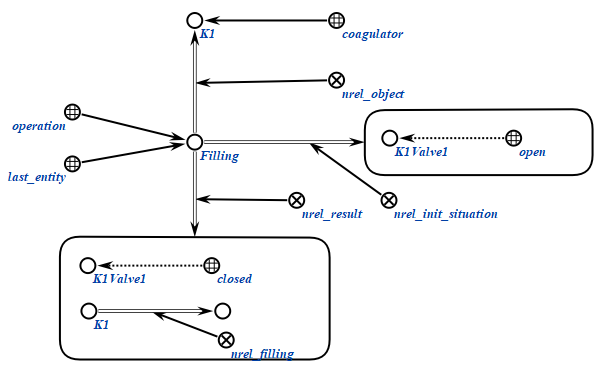
\includegraphics[scale=0.7]{./figures/sd_temp_entities/process_description.png}
		\end{figure}
	\end{SCn}
\end{frame}